% !TEX root = report.tex

\section{Experimental Results}
\label{sec:results}

\subsection{Overall Performance}

The hierarchical classifier wins on every test metric: 87.55\% top-1, 94.77\% top-5, and 0.870 macro F1. It exceeds the OverFeat baseline~\cite{Yang2015} by 4.65 percentage points. \tab{tab:main_results} gives the full comparison and \fig{fig:accuracy_comparison} plots top-1 against top-5 accuracy.

\begin{table}[ht]
\centering
\caption{Test Set Results for Make Classification (75 Classes). Precision, Recall and F1 are macro-averaged.}
\label{tab:main_results}
\small
\setlength{\tabcolsep}{3.5pt}
\begin{tabular}{lcccccc}
\toprule
\textbf{Model} & \textbf{Params} & \textbf{Top-1} & \textbf{Top-5} & \textbf{Prec.} & \textbf{Rec.} & \textbf{F1} \\
\midrule
SimpleCNN & 1.6M & 53.08 & 77.12 & 0.572 & 0.426 & 0.459 \\
ResNet50 (CE) & 24.6M & 82.28 & 91.88 & 0.839 & 0.769 & 0.789 \\
ResNet50 (Focal) & 24.6M & 80.39 & 91.12 & 0.830 & 0.742 & 0.763 \\
ResNet50 (LS) & 24.6M & 82.69 & 88.47 & 0.794 & 0.814 & 0.770 \\
EfficientNet-B0 & 4.1M & 86.95 & 94.50 & 0.897 & 0.833 & 0.853 \\
ResNet50-SE & 24.4M & 84.48 & 93.78 & 0.911 & 0.821 & 0.853 \\
\textbf{Hierarchical} & 25.9M & \textbf{87.55} & \textbf{94.77} & 0.910 & 0.849 & \textbf{0.870} \\
\midrule
OverFeat~\cite{Yang2015} & n/a & 82.90 & n/a & n/a & n/a & n/a \\
\bottomrule
\end{tabular}
\end{table}

\begin{figure}[ht]
\centering
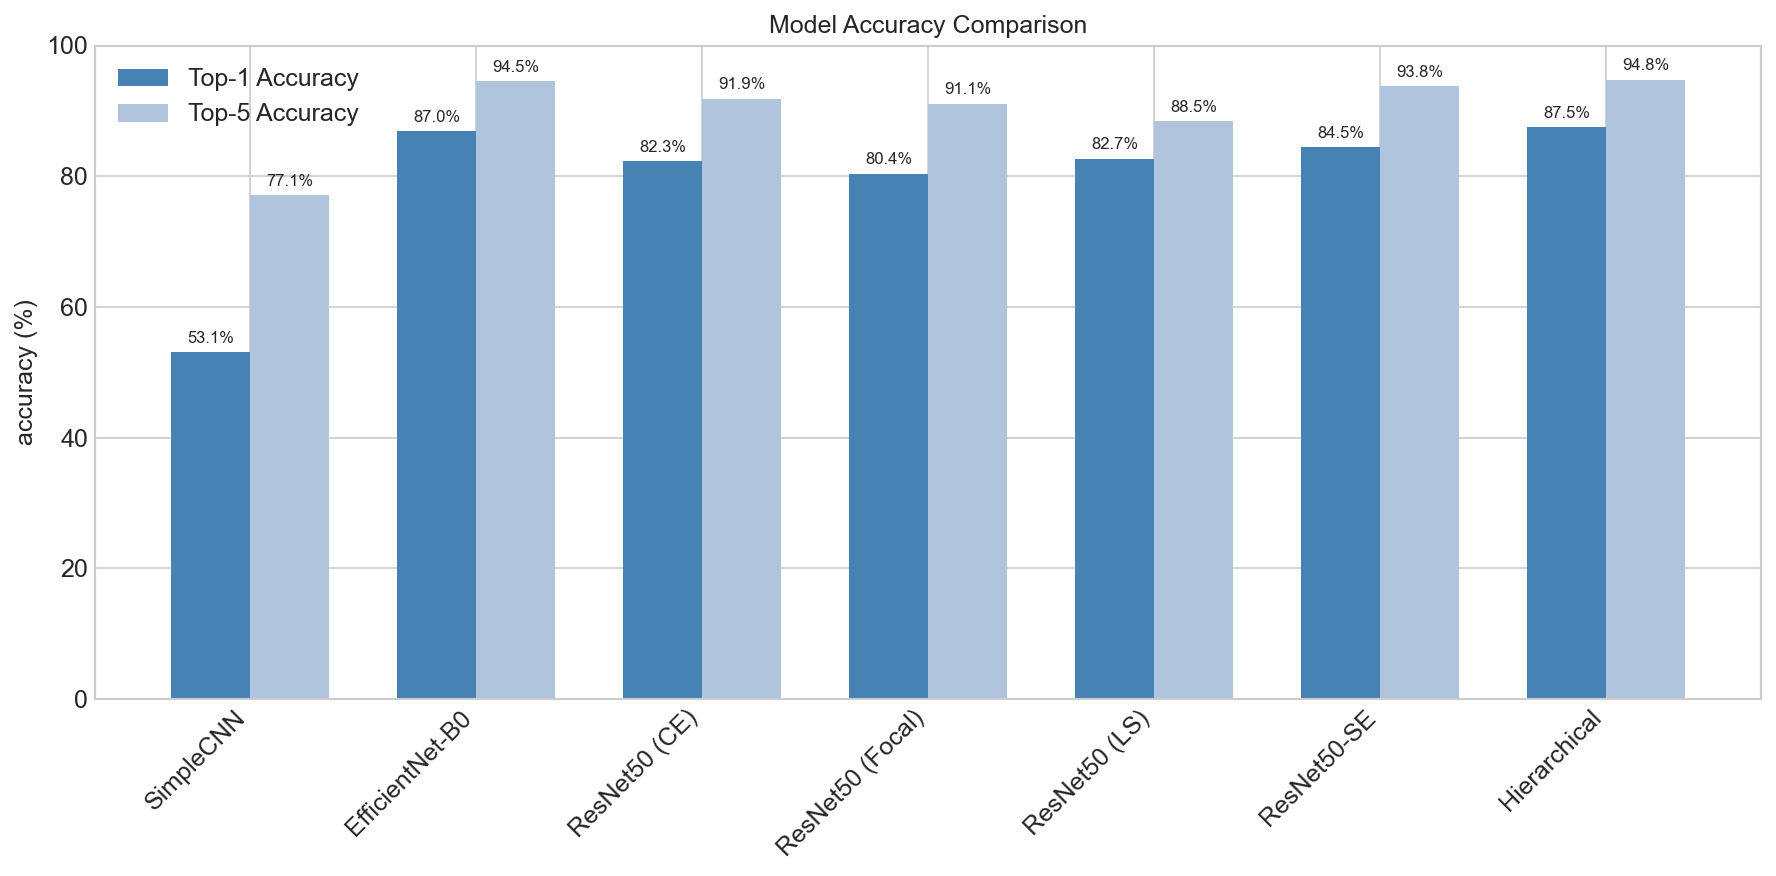
\includegraphics[width=\columnwidth]{figures/accuracy_comparison.png}
\caption{Top-1 and Top-5 accuracy comparison across all models.}
\label{fig:accuracy_comparison}
\end{figure}

Macro recall is consistently the weakest of the three averaged metrics, and it separates the models more than top-1 does. ResNet50-SE and the hierarchical model reach almost identical macro precision (0.911 against 0.910) but differ by 2.8 points of recall (0.821 against 0.849). The models are conservative on rare classes rather than wrong about them, which the per-class analysis below confirms.

\subsection{Impact of Transfer Learning}

Transfer learning is the single largest effect in the study. SimpleCNN, trained from scratch under the same schedule, reaches 53.08\% test accuracy against 80.39\% to 86.95\% for the pretrained backbones, a spread of 27 to 34 percentage points. Its macro F1 (0.459) is barely half that of any pretrained model.

The gap shows in the training dynamics as well. SimpleCNN converges more slowly and overfits harder, and its validation accuracy stalls at 74.78\% while training accuracy climbs to 85.80\%. Without ImageNet features the network has to learn edges, textures, and shape priors from 16k images, and it does not have enough data to do so.

\subsection{Architecture Comparison}

\subsubsection{Attention}

SE blocks lift ResNet50 with label smoothing from 82.69\% to 84.48\%, a gain of 1.79 points for 0.7M attention parameters. The larger gain is in macro precision, from 0.794 to 0.911, and in top-5 accuracy, from 88.47\% to 93.78\%. Channel recalibration mostly removes confident wrong answers rather than adding new correct ones.

\subsubsection{Parameter Efficiency}

EfficientNet-B0 reaches 86.95\% with 4.1M parameters. It beats the 24.6M-parameter ResNet50 (LS) by 4.26 points using 6$\times$ fewer parameters, and comes within 0.6 points of the hierarchical model at one sixth of its size. \fig{fig:acc_vs_params} shows the trade-off. Depthwise separable convolutions, compound scaling, and the SE attention built into every MBConv block all contribute; note that the built-in attention is consistent with the independent gain measured for ResNet50-SE.

\begin{figure}[ht]
\centering
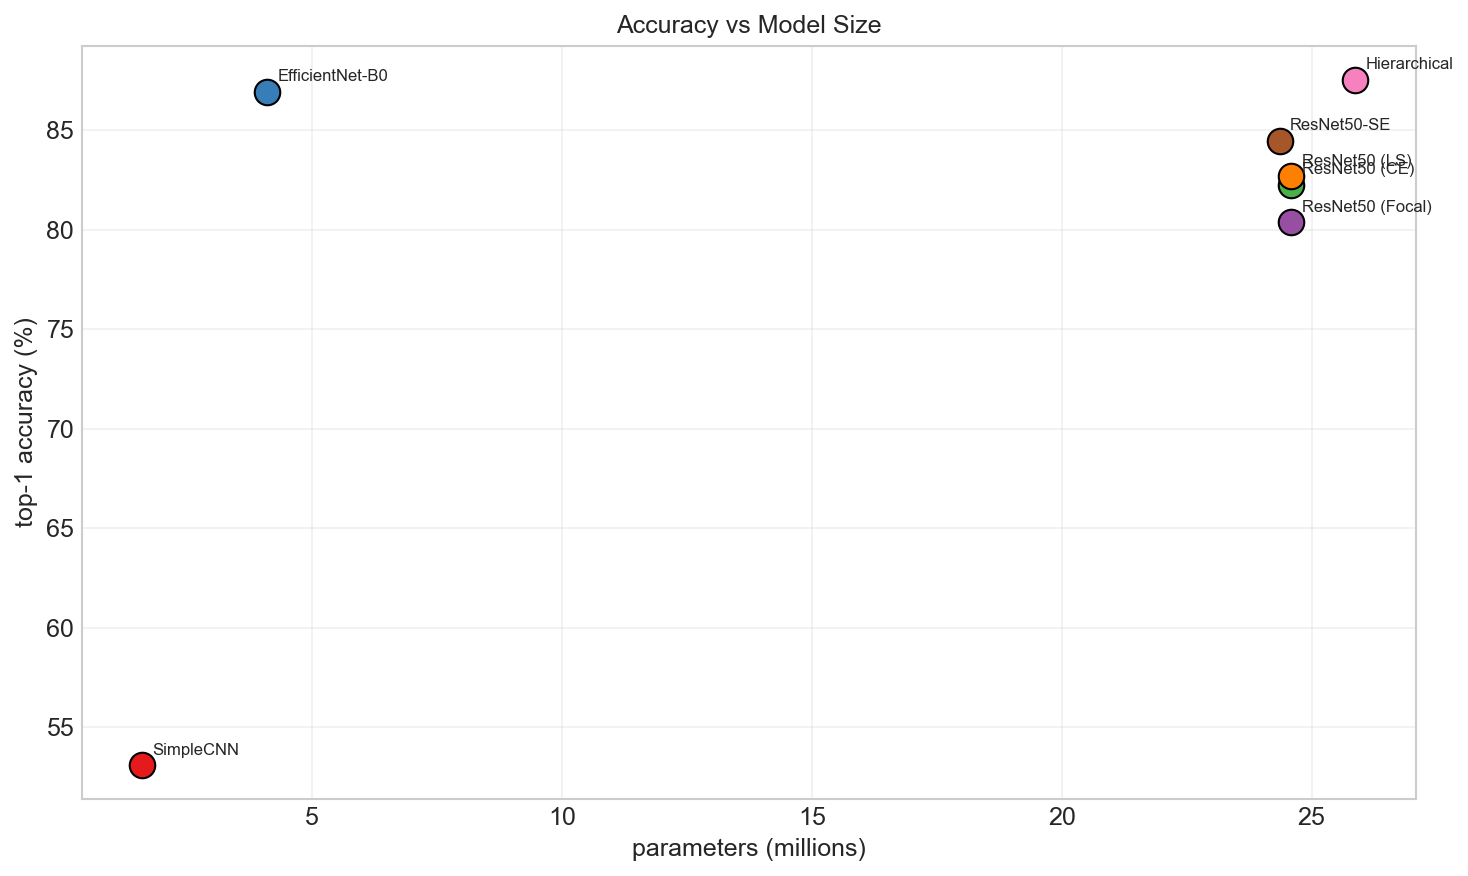
\includegraphics[width=\columnwidth]{figures/acc_vs_params.png}
\caption{Test accuracy against model size. EfficientNet-B0 is the efficiency winner.}
\label{fig:acc_vs_params}
\end{figure}

\subsection{Inference Cost}

Parameter count alone does not settle deployment. \tab{tab:timing} reports measured inference over the full 14,939-image test set at batch size 32 on an RTX 3060.

\begin{table}[ht]
\centering
\caption{Inference Cost (RTX 3060, batch size 32, 14,939 images)}
\label{tab:timing}
\begin{tabular}{lccc}
\toprule
\textbf{Model} & \textbf{Params} & \textbf{ms/image} & \textbf{Images/s} \\
\midrule
SimpleCNN & 1.60M & 0.58 & 1734 \\
EfficientNet-B0 & 4.10M & 1.18 & 844 \\
ResNet50 (CE) & 24.60M & 2.43 & 411 \\
ResNet50 (Focal) & 24.60M & 2.44 & 410 \\
ResNet50 (LS) & 24.60M & 2.46 & 406 \\
ResNet50-SE & 24.36M & 2.54 & 394 \\
Hierarchical & 25.87M & 2.38 & 420 \\
\bottomrule
\end{tabular}
\end{table}

EfficientNet-B0 sustains 844 images per second, roughly double any ResNet50 variant, while giving up 0.6 accuracy points to the best model. The SE blocks cost about 3.5\% throughput against ResNet50 (LS) for their 1.79-point gain. The second head of the hierarchical model is free at inference: 420 images per second, statistically indistinguishable from plain ResNet50, because the heads are trivial next to the shared backbone. If the make prediction is all that is needed, the model head can simply be discarded.

\subsection{Loss Function Comparison}

\tab{tab:loss_comparison} compares losses on ResNet50 with everything else held fixed. Focal loss ($\gamma$=2) loses 1.89 points to cross-entropy despite the 120:1 imbalance it is designed for. Label smoothing gains 0.41 points on top-1 but loses 3.41 points of top-5 accuracy (88.47\% against 91.88\%), so it is not a clear win either.

\begin{table}[ht]
\centering
\caption{Loss Function Comparison (ResNet50)}
\label{tab:loss_comparison}
\small
\setlength{\tabcolsep}{4pt}
\begin{tabular}{lcccc}
\toprule
\textbf{Loss Function} & \textbf{Val Acc} & \textbf{Test Top-1} & \textbf{Test Top-5} & \textbf{$\Delta$ Top-1} \\
\midrule
Cross-Entropy & 97.75\% & 82.28\% & 91.88\% & baseline \\
Focal ($\gamma$=2) & 96.69\% & 80.39\% & 91.12\% & -1.89 \\
Label Smoothing & 97.57\% & 82.69\% & 88.47\% & +0.41 \\
\bottomrule
\end{tabular}
\end{table}

The choice of loss is worth at most 2 points here, an order of magnitude less than the choice of backbone initialization. Focal loss down-weights the easy majority of examples, and on a dataset where the head classes are large but not pathological that mostly removes useful gradient signal. Imbalance is not the binding constraint on this task; the discriminability of the classes is.

\subsection{Training Dynamics}

\fig{fig:val_accuracy} and \fig{fig:val_loss} show validation accuracy and loss. All pretrained models are within a point of their peak by roughly epoch 20. Best validation accuracies: hierarchical 98.94\%, ResNet50-SE 98.00\%, EfficientNet-B0 and ResNet50 (CE) 97.75\%, ResNet50 (LS) 97.57\%, ResNet50 (Focal) 96.69\%, SimpleCNN 74.78\%.

Wall-clock training time for the full 100-epoch schedule ranged from 22 minutes (SimpleCNN) through 53 minutes (EfficientNet-B0) to roughly 1h22m for the ResNet50 family and 1h24m for the hierarchical model. The second head adds no meaningful training cost either.

\begin{figure}[ht]
\centering
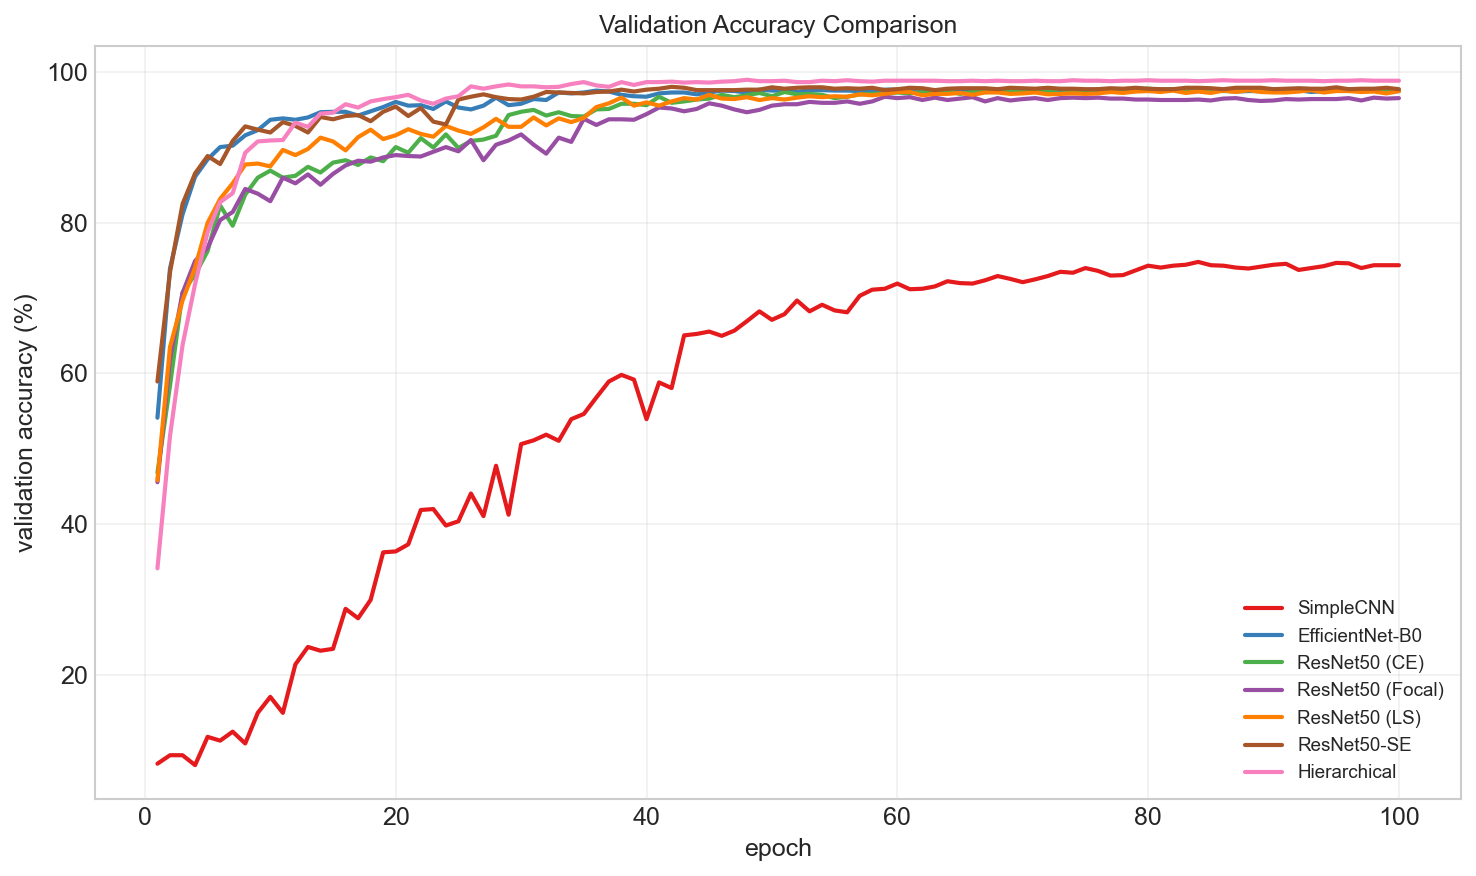
\includegraphics[width=\columnwidth]{figures/val_accuracy_overlay.png}
\caption{Validation accuracy during training for all models.}
\label{fig:val_accuracy}
\end{figure}

\begin{figure}[ht]
\centering
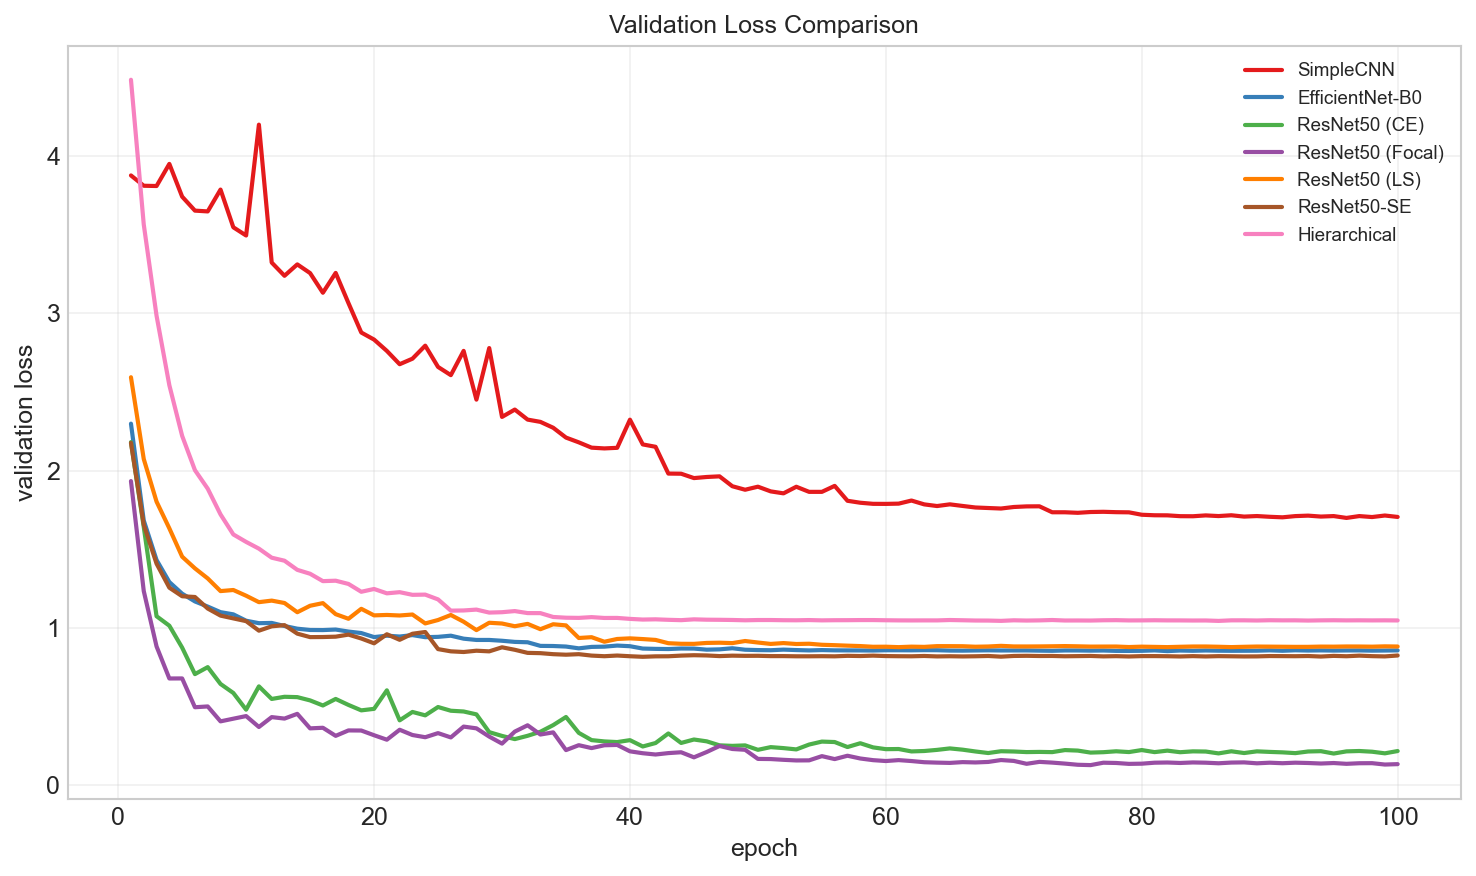
\includegraphics[width=\columnwidth]{figures/val_loss_overlay.png}
\caption{Validation loss during training for all models.}
\label{fig:val_loss}
\end{figure}

\subsection{Generalization Analysis}

Two gaps matter and they tell different stories. \tab{tab:gen_gap} reports both: the train-to-validation gap averaged over the last 10 epochs, and the validation-to-test gap at the best checkpoint. \fig{fig:gen_gap} shows the first throughout training.

\begin{table}[ht]
\centering
\caption{Generalization Gaps}
\label{tab:gen_gap}
\begin{tabular}{lccc}
\toprule
\textbf{Model} & \textbf{Train-Val} & \textbf{Best Val} & \textbf{Val-Test} \\
 & \textbf{(last 10 ep.)} & & \textbf{gap} \\
\midrule
SimpleCNN & 11.48\% & 74.78\% & 21.70\% \\
EfficientNet-B0 & 2.47\% & 97.75\% & 10.80\% \\
ResNet50 (CE) & 2.38\% & 97.75\% & 15.47\% \\
ResNet50 (Focal) & 3.52\% & 96.69\% & 16.30\% \\
ResNet50 (LS) & 2.62\% & 97.57\% & 14.88\% \\
ResNet50-SE & 2.22\% & 98.00\% & 13.52\% \\
\textbf{Hierarchical} & \textbf{1.18\%} & 98.94\% & \textbf{11.39\%} \\
\bottomrule
\end{tabular}
\end{table}

\begin{figure}[ht]
\centering
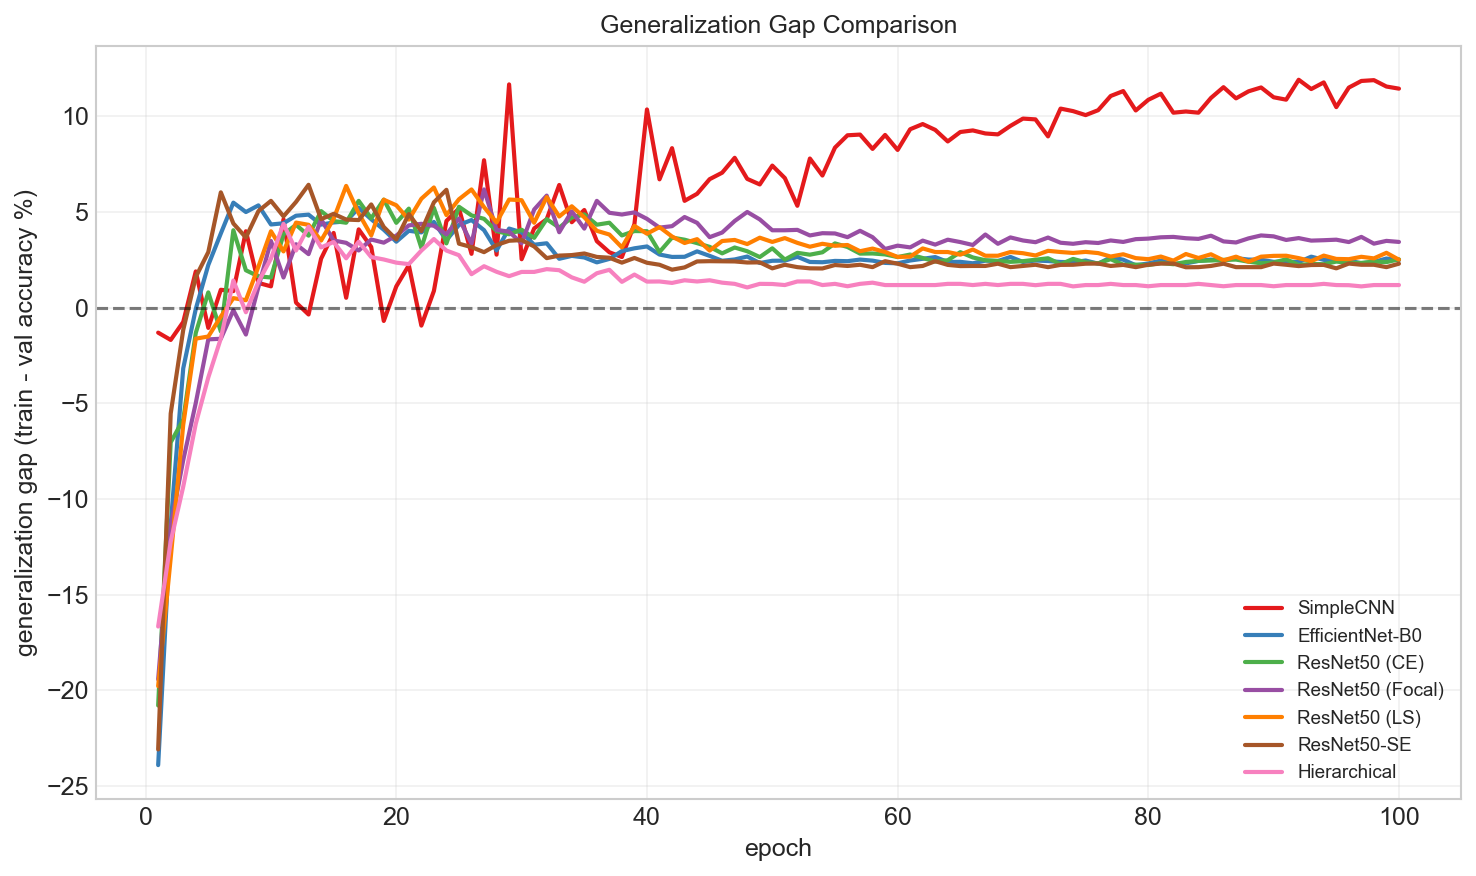
\includegraphics[width=\columnwidth]{figures/generalization_gap_overlay.png}
\caption{Train-to-validation accuracy gap throughout training. SimpleCNN diverges; the pretrained models stay flat.}
\label{fig:gen_gap}
\end{figure}

SimpleCNN's train-to-validation gap grows monotonically to 11.48\%: training accuracy keeps rising while validation accuracy flattens after roughly epoch 30. That is textbook memorization on insufficient data.

The pretrained models all sit between 1.18\% and 3.52\%, so by the train-to-validation measure they look well regularized. The validation-to-test gap contradicts that. Every model loses 10 to 22 points moving from validation to test. This is the most important negative result in the study and it is a property of the data, not of the models: the validation split is a random 10\% of the training images, so it shares photo sources, sessions, and backgrounds with the training set, while the official test split does not. Validation accuracy on this dataset is not a usable estimate of test accuracy, only a usable signal for model selection.

The ranking of the val-test gap is still informative. The hierarchical model (11.39\%) and EfficientNet-B0 (10.80\%) leak least; focal loss leaks most among the pretrained models (16.30\%).

\subsection{Per-Class Behaviour}

Aggregate accuracy hides where the errors sit. On the hierarchical model's make head, per-class F1 correlates with class size but weakly: mean F1 is 0.853 for the 23 makes with fewer than 50 test images, 0.873 for the 22 makes between 50 and 199, and 0.883 for the 30 makes with 200 or more. Nine makes fall below 0.80 F1 and seven reach 0.95 or above.

The failure mode is recall, not precision. The worst class has precision 1.00 and recall 0.39: when the model names it, it is right, but it names it rarely. The largest class in the test set (1,125 images) shows the opposite profile, precision 0.70 against recall 0.97, absorbing predictions that belong elsewhere.

That asymmetry is visible in \tab{tab:confusions}, which lists the top confusion pairs per model. Volkswagen is the sink: it is the predicted label in 7 of the hierarchical model's 10 worst confusion pairs, and 15.9\% of all Skoda test images are called Volkswagen by EfficientNet-B0 (8.8\% by the hierarchical model). This is not a modelling artefact. Skoda is a Volkswagen Group marque and shares platforms and styling language with it, and Volkswagen is the largest class in the dataset, so the prior and the visual evidence point the same way. The other recurring pairs (Zhonghua, Geely, Buck, GreatWall, Jianghuai into Volkswagen) are Chinese makes whose designs of that era borrowed heavily from the Volkswagen visual idiom.

\begin{table}[ht]
\centering
\caption{Top Confusion Pairs, Hierarchical Model}
\label{tab:confusions}
\begin{tabular}{llcc}
\toprule
\textbf{True} & \textbf{Predicted} & \textbf{Count} & \textbf{\% of true class} \\
\midrule
Skoda & Volkswagen & 25 & 8.8 \\
Zhonghua & Volkswagen & 16 & 7.1 \\
Buck & Volkswagen & 11 & 2.5 \\
Geely & Volkswagen & 9 & 4.9 \\
BYD & Haima & 9 & 4.3 \\
Citroen & Volkswagen & 9 & 2.6 \\
Volkswagen & Audi & 8 & 0.7 \\
Benz & Volkswagen & 8 & 1.3 \\
Jianghuai & Volkswagen & 8 & 3.3 \\
GreatWall & Volkswagen & 8 & 4.2 \\
\bottomrule
\end{tabular}
\end{table}

The single most extreme case in the study is EfficientNet-B0 calling 66.7\% of Brabus images Benz. Brabus is a Mercedes-Benz tuner, so those images are Mercedes bodies. The label is correct and the model is not seeing anything the pixels do not contain. This is a limit of make classification from a single image, not a fixable error.

\subsection{Hierarchical Model Analysis}

The multi-task model is the only one evaluated on both tasks. \tab{tab:hier} reports both heads on the test set.

\begin{table}[ht]
\centering
\caption{Hierarchical Model, Both Heads (Test Set)}
\label{tab:hier}
\begin{tabular}{lccc}
\toprule
\textbf{Head} & \textbf{Top-1} & \textbf{Top-5} & \textbf{Macro F1} \\
\midrule
Make (75 classes) & 87.55\% & 94.77\% & 0.870 \\
Model (431 classes) & 82.72\% & 91.80\% & 0.819 \\
\midrule
OverFeat make~\cite{Yang2015} & 82.90\% & n/a & n/a \\
OverFeat model~\cite{Yang2015} & 76.70\% & n/a & n/a \\
\bottomrule
\end{tabular}
\end{table}

The 431-class model head reaches 82.72\% top-1, which exceeds the OverFeat model-classification baseline (76.7\%) by 6.02 points, a larger margin than on the make task. A single network therefore beats the reference on both levels of the hierarchy at once.

The two heads fail together. Of the 2,582 test images where the model head is wrong, 60.0\% also have the make wrong. Conversely, of the 1,860 images where the make head is wrong, the model head still gets the exact car model right 16.8\% of the time, which means the shared features carry model identity that the make head fails to exploit on those images. The errors are correlated but not identical, which is exactly the condition under which the auxiliary task supplies useful gradient rather than a duplicate of the primary one.

The regularization effect is measurable. The hierarchical model has the lowest train-to-validation gap (1.18\% against 2.22\% for the next best) and the second-lowest val-test gap, while carrying the most parameters of any model tested. Forcing the backbone to also separate 431 models leaves it less free to memorize the 75-way make task.

\emph{Correction to a common reading of these numbers.} The validation figures for the hierarchical model (98.94\% make, 95.51\% model) are not test figures and should not be quoted as such. Test performance is 87.55\% and 82.72\%. The gap between the two is the val-test leak discussed above.

\subsection{Comparison to Baseline}

The hierarchical model exceeds OverFeat by 4.65 points on make and 6.02 points on model. The improvement is attributable to four things, in rough order of contribution:

\begin{enumerate}
    \item Residual architectures and stronger ImageNet pretraining, which the transfer-learning ablation shows to be worth 27 to 34 points on their own.
    \item The multi-task formulation, worth 4.86 points over the ResNet50 (LS) single-task model with the same backbone.
    \item Attention, worth 1.79 points in isolation.
    \item Training technique (AdamW, differential learning rates, label smoothing, AMP), worth under 1 point measurably.
\end{enumerate}
